\documentclass[12pt]{article}

% --- Packages ---
\usepackage{graphicx}   % images
\usepackage{caption}    % nicer captions
\usepackage{geometry}   % margins
\usepackage{float}      % [H] placement
\usepackage[hidelinks]{hyperref} % clickable links (optional)

% --- Page setup ---
\geometry{margin=1in}
\setlength{\parskip}{0.6em}
\setlength{\parindent}{0pt}

% --- Where images live (relative to docs/) ---
\graphicspath{{../renders/}}

% --- Title info ---
\title{\textbf{Starship CAD Project} \\
       \large AME 5193: Intro to Computer-Aided Design}
\author{Blake Thomas Johnson}
\date{Spring 2025}

\begin{document}

\maketitle

\begin{figure}[H]
    \centering
    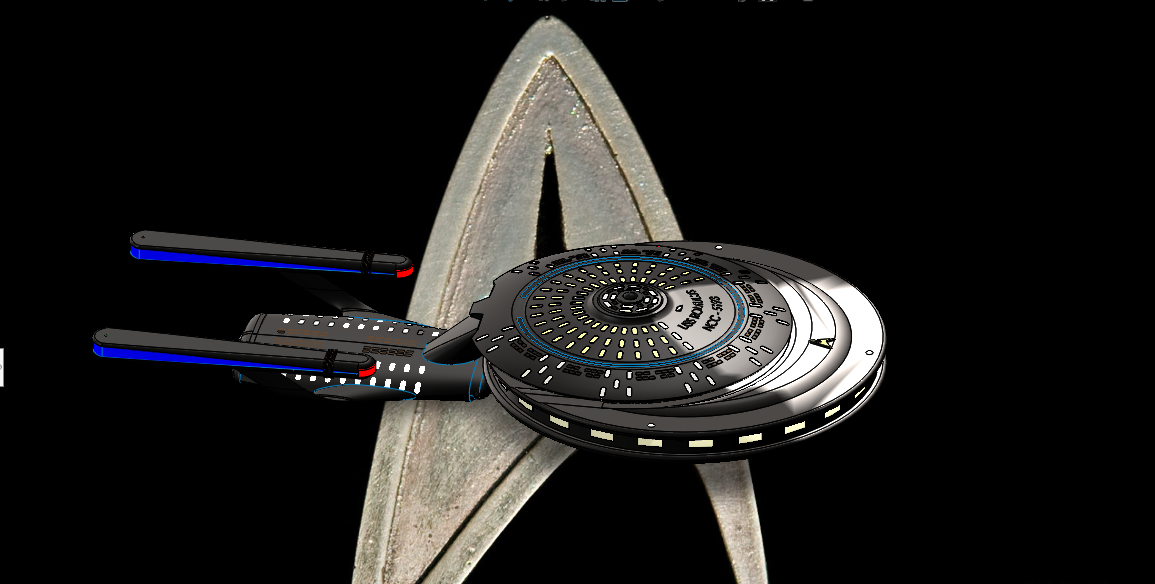
\includegraphics[width=0.78\textwidth]{final_1.png}
    \caption{Overall starship render (final configuration).}
\end{figure}

\clearpage

\section*{Executive Summary}
This document summarizes the parametric design and assembly of a Starfleet-inspired
starship created in SolidWorks. Key objectives included modular subsystem architecture,
constraint-driven assemblies (mates), symmetry and patterning for efficient iteration,
and presentation-quality renders. The deliverables comprise a complete assembly,
neutral exports (STEP/STL), and a concise portfolio summary intended for non-CAD
reviewers.

\section*{Design Objectives}
\begin{itemize}
    \item Apply parametric, modular design principles to saucer, engineering hull, and nacelles.
    \item Use symmetry planes, feature patterns, and fillet strategy to reduce model complexity.
    \item Build robust assembly mates for repeatable alignment and motion constraints.
    \item Produce clear visuals and lightweight exports for recruiter-friendly review.
\end{itemize}

\section*{System Overview}
\begin{figure}[H]
    \centering
    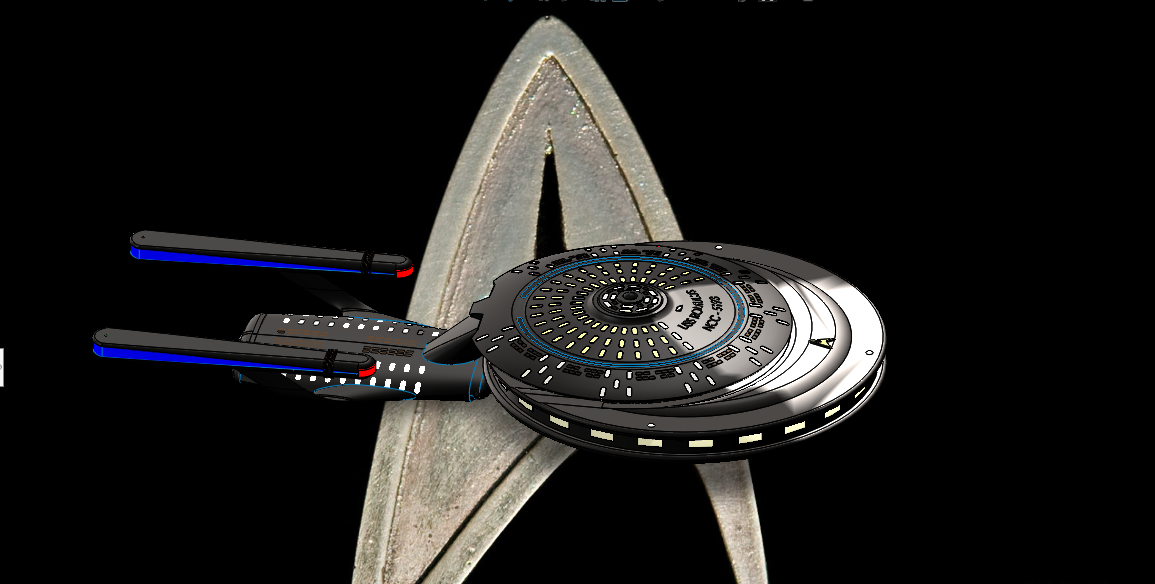
\includegraphics[width=0.82\textwidth]{final_1.png}
    \caption{Overall assembly highlighting saucer, engineering section, and twin nacelles.}
\end{figure}

\begin{figure}[H]
    \centering
    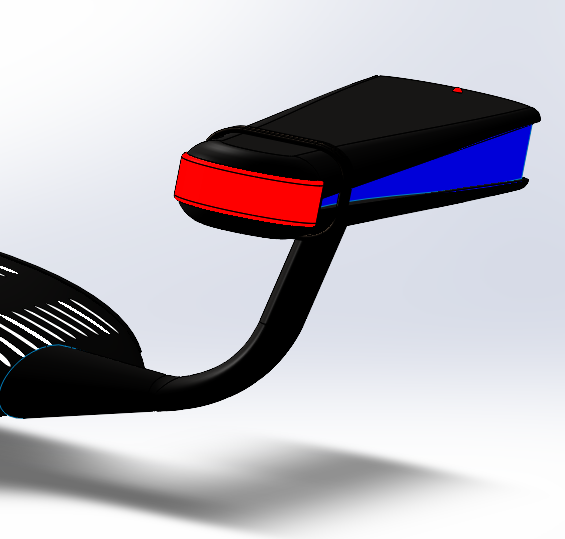
\includegraphics[width=0.82\textwidth]{sleek.png}
    \caption{Profile view emphasizing streamlined geometry and symmetry.}
\end{figure}

\section*{Subsystem Highlights}

\subsection*{Command Module}
\begin{figure}[H]
    \centering
    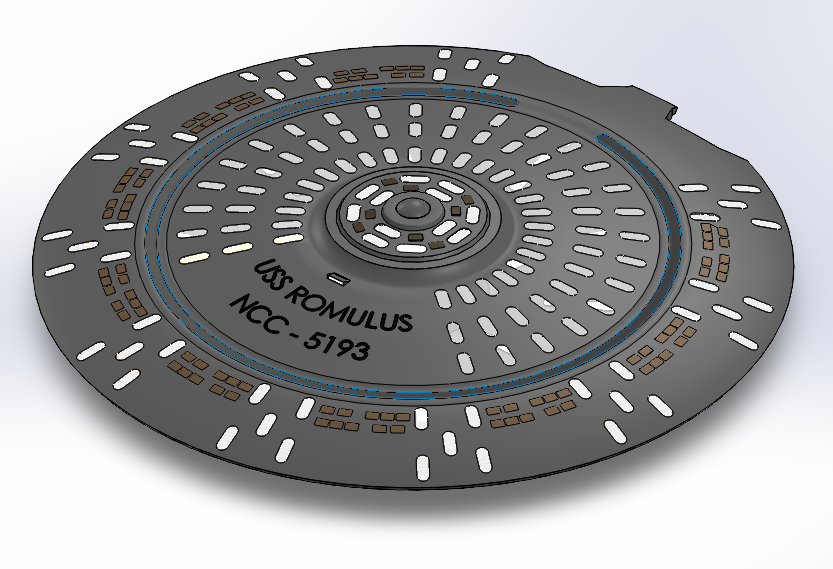
\includegraphics[width=0.7\textwidth]{command.png}
    \caption{Command/bridge section with forward modules and canopy geometry.}
\end{figure}
Design intent: clean loft transitions, curvature continuity, and alignment to the ship
centerline. Interfaces defined to mate reliably with saucer section.

\subsection*{Engineering Section}
\begin{figure}[H]
    \centering
    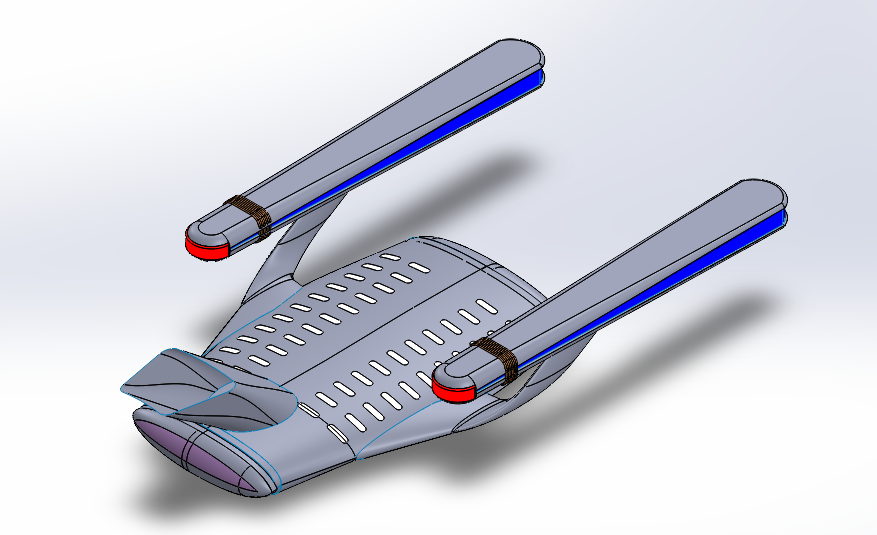
\includegraphics[width=0.7\textwidth]{engineering.png}
    \caption{Engineering hull with internal volume for propulsion and docking interfaces.}
\end{figure}
Design intent: structural backbone tying saucer and nacelles, with consistent fillet
hierarchy and accessible mounting planes.

\subsection*{Nacelles}
\begin{figure}[H]
    \centering
    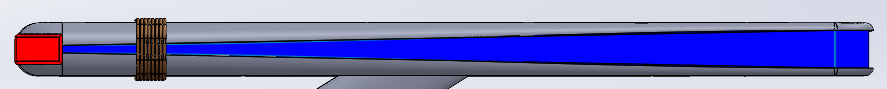
\includegraphics[width=0.7\textwidth]{nacelles.png}
    \caption{Nacelle details and pylons; attachment features ensure repeatable alignment.}
\end{figure}
Design intent: mirrored components driven by common parameters; pylon thickness and
angles set by reference geometry for quick iteration.

\subsection*{Detail Example}
\begin{figure}[H]
    \centering
    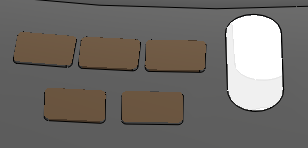
\includegraphics[width=0.7\textwidth]{windows_epods.png}
    \caption{Window/e-pod details providing scale cues and surface interest.}
\end{figure}

\section*{CAD Implementation}
Software: \textbf{SolidWorks} (version \emph{fill in}). Units: meters. Core techniques:
reference planes for symmetry, sketch constraints for intent, feature patterns for
repeated elements, and consistent fillet/edge treatment. Assembly uses primary mates
(planes, axes) first, followed by local mates at interfaces. Neutral exports (STEP/STL)
are provided for viewing without CAD.

\section*{Conclusion}
The project demonstrates CAD modeling discipline, subsystem integration, and clear
technical communication. The model’s parametric structure supports rapid changes,
while curated renders and neutral exports make the work accessible to reviewers.


\end{document}



